\section{Virtual Private Networks}

\subsection{Overview}

\paragraph{VPN}
A VPN creates a secure channel between two private networks over an untrusted, public network (the Internet) - this provides security on the link / network layer. Additionally, functionality and management of the private network can be transferred to the established VPN.

A VPN can connect physically separated networks (site-to-site), connect a remote host to a company/university network (host-to-site), circumvent censorship, avoid tracking, hide user's IP address, spoof locations, allow access to restricted content, etc.

A VPN provider has access to metadata of all traffic - anonymity is not given.

\paragraph{Part 1: Set-Up Phase}
The tunnel endpoints authenticate each other and set up keys (similar to the TLS handshake).

\paragraph{Part 2: Tunneling Phase}
Packets are encapsulated and decapsulated at the endpoints. Additionally, the original data is encrypted and authenticated with a MAC.

\paragraph{VPN Tunnel Properties}
A VPN tunnel holds similar security properties as the TLS Record Protocol (source authentication, data integrity, confidentiality, replay suppression, etc.). However, some tunneling protocols do not provide encryption/authentication.

\paragraph{VPN vs. TLS}
\begin{itemize}
    \item VPN protects all kinds of traffic (e.g. DNS requests, etc.).
    \item Services in private networks / behind firewalls can be accessed with VPNs.
    \item VPN data is only secure in the tunnel. TLS protects data end-to-end.
    \item VPN servers can see unencrypted traffic (here, TLS is still necessary).
    \item A web server cannot be authenticated with VPN, only the tunnel endpoint.
    \item TLS does not authenticate clients.
    \item VPN utilize many different protocols.
    \item TLS is commonly used on top of a VPN.
\end{itemize}

\paragraph{Performance / Availability}
VPNs introduce overhead with additional cryptographic operations, potential detours and limited bandwidth at VPN servers. There is no built-in defense against (D)DoS and routing attacks, therefore VPNs do not provide a higher availability. Packet filtering targeting VPN packets would need to target all VPN packets since content is hidden.

\paragraph{VPN vs. VLAN}
A VPN connects two different networks, resulting in one virtual network over multiple physical ones. VLANs set up multiple isolated virtual networks (logical groupings) on a single physical infrastructure. VLANs are often used in cloud-computing environments to isolate communication between VMs or to form multiple broadcast domains in a network with frequent broadcasts. VLANs do not provide authentication. A virtual extensible LAN (VXLAN) combines both features.

VLANs are L2 constructs, analogous to IP subnets which are L3 constructs. There is often a one-to-one relationship between a VLAN and an IP subnet (it is possible to have multiple subnets on one VLAN).

\paragraph{Implementing VPN Functionality}
There are many different protocols and applications that implement VPN functionality. They can differ in authentication mechanisms (PSK, PKI, etc.), the tunnel protocol (custom ones, SSTP, etc.), the inner protocol = outermost header of an encapsulated packet (network vs. link layer VPN - e.g. IPsec L3, WireGuard L2, etc.) and of course how they're implemented (in user space, a kernel module, directly in hardware, etc.).

\paragraph{Endpoints at Hosts}
A VPN creates virtual network adapters (e.g. "eth2", "tun0", etc.) at the end hosts, one route with the public IP of the VPN server as a destination and a new default route to the private address of the VPN tunnel. They can be used like any other network adapter and one can either send all traffic through it or selectively (\textit{split tunnel}) by choosing only a subset of IP prefixes that should use the VPN. %TODO image? see notes


\subsection{VPN Implementations}

\paragraph{IPsec}
IPsec is a secure network protocol suite (very large, many options / modes) that authenticates and encrypts packets over an IP network - also supports data integrity and replay protection. There is mutual authentication between agents at the beginning of a session along with negotiation of keys to use during it. Problems include difficult configuration due to many options where some don't even provide security (no encryption and no authentication) and the possibility of insecure ciphers (similar to TLS problems).

\textbf{Comparison to TLS:} In HTTPS, client certificate authentication is rare while in IPsec it is the norm. This is because websites are usually publicly accessible while private networks apply strong restriction on authorized users. IPsec explicitly includes sequence numbers in its packets since IP is only best-effort (loss, reordering, duplication) while TLS maintains only local counters since it runs on top of TCP.


\begin{figure}[h]
	\centering
	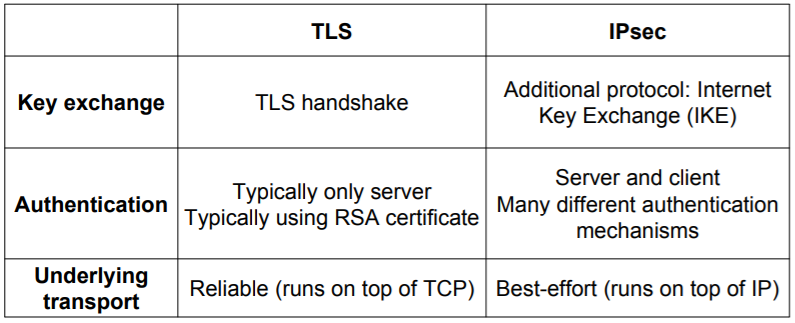
\includegraphics[scale=0.6]{images/5-ipsec_tls.PNG}
	\caption{Comparison of TLS and IPsec.}
	\label{fig:ipsec_tls}
\end{figure}

\textbf{Typical Session:} first set up a security association (SA) via Internet Key Exchange (IKE) and then encapsulate packets and tunnel them between SA endpoints with Encapsulation Security Payload (ESP).

\textbf{IKEv2:} first establish a temporary and anonymous key for the rest of the IKE exchange and then authenticate each other by sending identity, (certificate), sig (asym.) / MAC (sym.), etc. (see Figure \ref{fig:ike}). Passive attacks cannot uncover the identities but an active MITM attack might. In case of ephemeral DH values at the beginning, we have perfect forward security. %TODO: how exactly?

\begin{figure}[h]
	\centering
	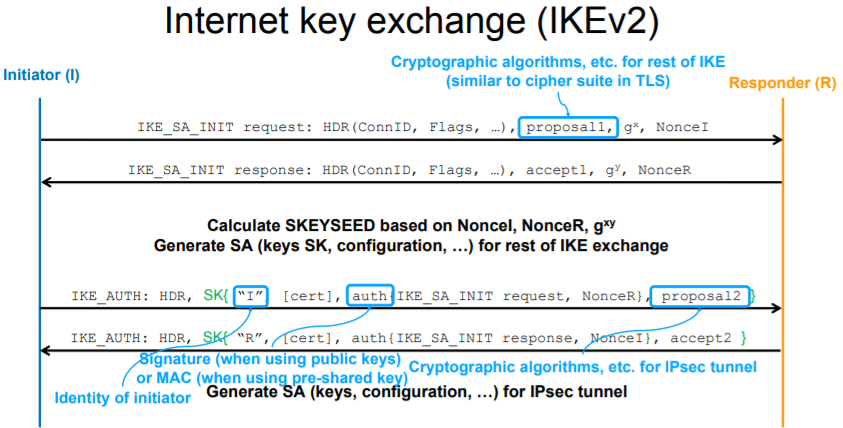
\includegraphics[scale=0.7]{images/5-ike.PNG}
	\caption{Simplified overview of the IKEv2.}
	\label{fig:ike}
\end{figure}

\textbf{ESP:} the original IP packet is first padded with the ESP trailer that also includes the type of the original packet (appended at the end). It is then fully encrypted. Then, the ESP header is added which includes the SA identification and a sequence number (replay protection, nonce for certain encryption algos, etc.). Lastly, an Integrity Check Value (ICV) is created and appended at the end - it is a MAC over the entire packet. Finally, a new IP header is added.

\textbf{Other Options:} there can be additional messages in IKEv2 (EAP, cookies, etc.) and other modes like the transport mode for end-to-end connections or an Authenticated Header (AH) protocol instead of ESP if we only want authentication but no encryption.

\paragraph{WireGuard}
Much faster and smaller than other options (IPsec, OpenVPN, etc.) by removing cryptographic agility, i.e. only support chosen state-of-the-art primitives (single cipher suite) s.t. negotiation is simplified and insecure primitives are removed. Configuration is kept simple. Attack surface is minimal by keeping the codebase small (also makes formal verification easier). L3 packets are encapsulted and transformed into L4 UDP only packets.

\textbf{Key Exchange and Authentication:} the WireGuard handshake follows the Noise Protocol Framework built exclusively on elliptic-curve DH exchanges. First, each peer has a static key pair (public and private) and specify in configuration which public keys are authorized. Each peer then creares an ephemeral key pair (public and private). The symmetric keys are then derived from four DH combinations (two static public key and two ephemeral public keys). See Figure \ref{fig:wireguard}. Since WireGuard is connectionless, a series of timers (based on message counts and time) are used to steer handshakes, key renegotiation and session termination. Perfect forward security is guaranteed with strict key rotation timers and the ephemeral ECDH session key exchange.

\begin{figure}[h]
	\centering
	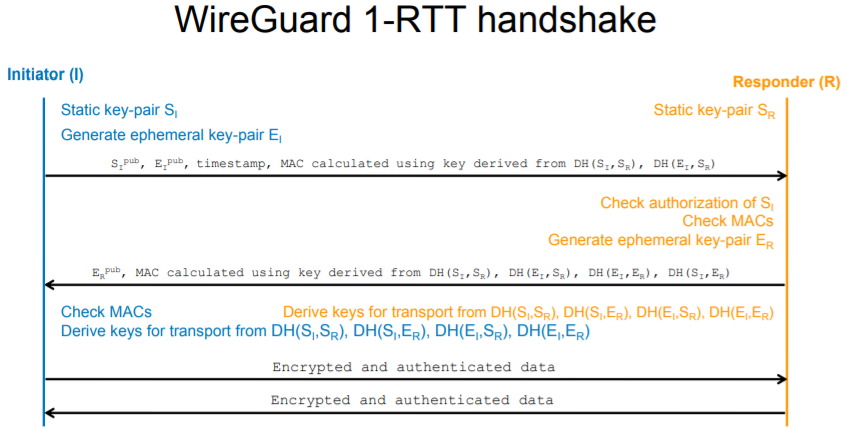
\includegraphics[scale=0.7]{images/5-wireguard.PNG}
	\caption{Simplified overview of the WireGuard handshake.}
	\label{fig:wireguard}
\end{figure}

\textbf{DoS Protection:} When under load, WireGuard can choose to respond with a cookie instead of processing the handshake (expensive cryptography). With this cookie, the initiator uses it as a key for computing HMACs of their message (similar to IKEv2 cookie-mode). Difference to IKEv2 cookie-mode is that an additional MAC is required on the handshake message (responder public key as HMAC key). Responder can stay completely silent unless initiator knows its public key. %TODO DoS protection in WireGuard and IPsec

%TODO if time, look at these
\paragraph{Point-To-Point Tunneling Protocol (PPTP)}

\href{https://citeseerx.ist.psu.edu/viewdoc/download?doi=10.1.1.503.7298&rep=rep1&type=pdf}{Comparison PPTP, L2TP, IPsec, etc.}

\paragraph{Generic Routing Encapsulation (GRE)}

\paragraph{Layer-2 Tunneling Protocol (L2TP)}

\paragraph{OpenVPN}

\paragraph{Secure Socket Layer (SSL)}

\paragraph{Secure Socket Tunneling Protocol (SSTP)}




\subsection{Summary}

\begin{itemize}
    \item VPNs create secure channels on the network/link layer.
    \item VPNs and end-to-end security (TLS) complement each other.
    \item There are many different VPN protocols and applications.
\end{itemize}